\section{Đặt vấn đề}

Trong bối cảnh chuyển đổi số và sự phát triển mạnh mẽ của cuộc cách mạng công nghiệp 4.0, các hệ thống nhúng và Internet of Things (IoT) đang ngày càng được ứng dụng rộng rãi trong nhiều lĩnh vực như sản xuất thông minh, giám sát môi trường, quản lý năng lượng và tự động hóa công nghiệp. Các hệ thống này không chỉ yêu cầu khả năng thu thập và xử lý dữ liệu theo thời gian thực mà còn đòi hỏi tính ổn định, khả năng mở rộng và mức độ bảo mật cao trong suốt quá trình vận hành.

Tuy nhiên, nhiều nền tảng nhúng hiện nay vẫn phụ thuộc vào các giải pháp đóng hoặc thiếu khả năng tùy biến sâu theo yêu cầu thực tế của từng hệ thống. Đối với các thiết bị biên (Edge Device), việc tối ưu tài nguyên phần cứng, kiểm soát thành phần phần mềm và đảm bảo khả năng vận hành ổn định là những yêu cầu đặc biệt quan trọng. Bên cạnh đó, sự gia tăng của các nguy cơ tấn công mạng, giả mạo firmware hoặc thay đổi dữ liệu trái phép cũng đặt ra yêu cầu cần có các cơ chế bảo vệ tính toàn vẹn và bảo mật cho hệ thống nhúng.

Trong lĩnh vực quản lý kho và giám sát môi trường công nghiệp, việc theo dõi các thông số như nhiệt độ, độ ẩm và trạng thái vận hành đóng vai trò quan trọng nhằm đảm bảo chất lượng lưu trữ hàng hóa, lương thực và thực phẩm. Các hệ thống giám sát truyền thống thường tồn tại nhiều hạn chế như khả năng mở rộng thấp, khó tùy biến hoặc phụ thuộc vào nền tảng phần mềm riêng biệt. Do đó, việc nghiên cứu và xây dựng một nền tảng Linux Embedded có khả năng tùy biến, hỗ trợ giao tiếp IoT và tích hợp các cơ chế bảo mật là cần thiết nhằm đáp ứng nhu cầu thực tế của các hệ thống công nghiệp hiện đại.

\begin{figure}[H]
    \centering
    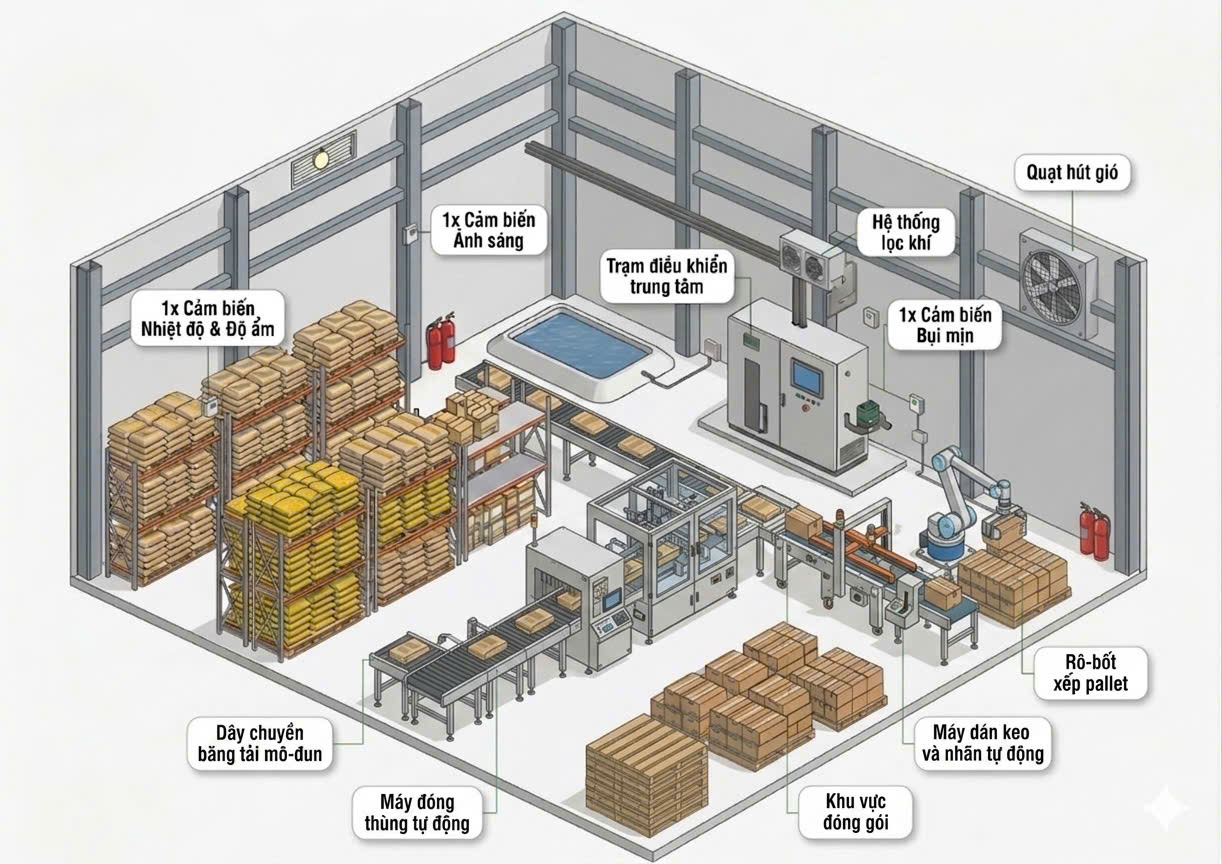
\includegraphics[width=0.8\linewidth]{image/baitoan.jpg}
    \caption{Mô hình bài toán đặt ra}
    \label{fig:placeholder}
\end{figure}

\section{Lý do chọn đề tài}

Yocto Project là nền tảng mã nguồn mở mạnh mẽ cho phép xây dựng và tùy biến hệ điều hành Linux nhúng theo từng kiến trúc phần cứng và yêu cầu ứng dụng cụ thể. Khác với các bản phân phối Linux truyền thống, Yocto cung cấp khả năng kiểm soát chi tiết các thành phần hệ thống, tối ưu tài nguyên và chủ động trong quá trình phát triển Embedded Linux Image.\cite{yocto_project_overview}

Bên cạnh khả năng tùy biến hệ thống, Yocto Project còn hỗ trợ tích hợp nhiều cơ chế bảo mật hiện đại như Secure Boot, dm-verity và fscrypt nhằm tăng cường tính toàn vẹn và độ an toàn cho hệ thống nhúng. Đây là những yếu tố đặc biệt quan trọng trong các hệ thống công nghiệp và IoT, nơi thiết bị thường hoạt động liên tục trong thời gian dài và yêu cầu độ ổn định cao.

Ngoài ra, việc phát triển các Linux Device Driver và tích hợp giao tiếp phần cứng trong môi trường Yocto cũng giúp tăng khả năng làm chủ hệ thống ở mức thấp, đồng thời tạo điều kiện thuận lợi cho việc nghiên cứu kiến trúc Linux Embedded một cách toàn diện hơn.

Xuất phát từ những yêu cầu thực tế trong lĩnh vực IoT và tự động hóa công nghiệp, đề tài được thực hiện nhằm nghiên cứu và xây dựng một nền tảng nhúng đa chức năng dựa trên Yocto Project, có khả năng tích hợp các cơ chế bảo mật, hỗ trợ giao tiếp thiết bị và phục vụ triển khai các ứng dụng giám sát công nghiệp. Trên cơ sở đó, đề tài triển khai bài toán giám sát kho thông minh như một mô hình ứng dụng thực tế để đánh giá tính ổn định, khả năng mở rộng và hiệu quả vận hành của hệ thống.

\begin{figure}[H]
    \centering
    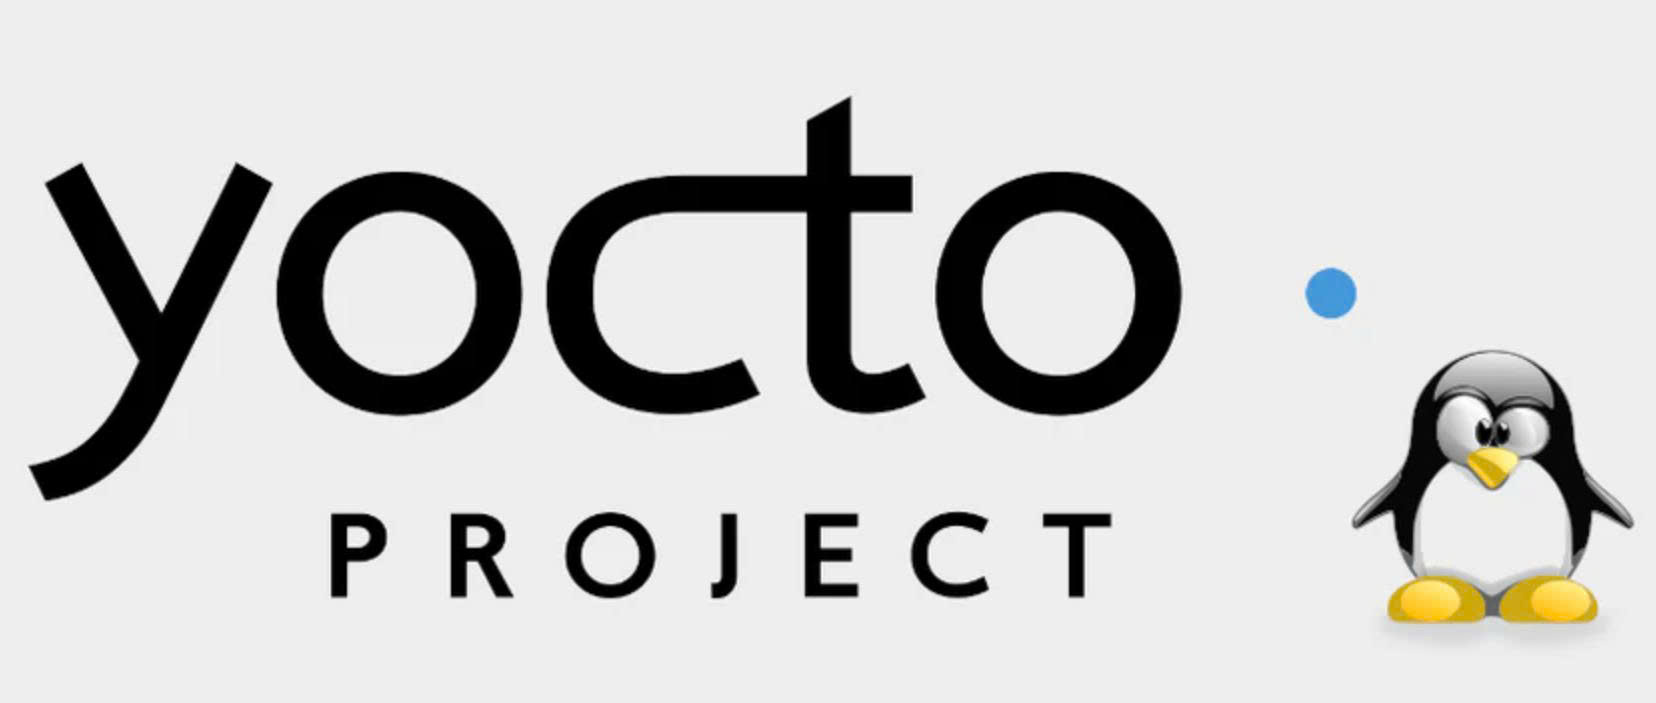
\includegraphics[width=0.5\linewidth]{image/yoctoc1.png}
    \caption{Nền tảng Yocto Project}
    \label{fig:placeholder}
\end{figure}

\section{Mục tiêu nghiên cứu}

Đề tài hướng đến mục tiêu nghiên cứu và xây dựng nền tảng Linux Embedded phục vụ cho các ứng dụng công nghiệp và IoT dựa trên Yocto Project. Hệ thống được thiết kế theo hướng tùy biến, có khả năng mở rộng và đáp ứng yêu cầu vận hành ổn định trên các thiết bị nhúng tài nguyên hạn chế.

Bên cạnh đó, đề tài tập trung nghiên cứu cơ chế xây dựng và tích hợp Linux Device Driver nhằm hỗ trợ giao tiếp phần cứng trong hệ thống nhúng. Các cơ chế quản lý module, Device Tree và tích hợp driver trong Yocto cũng được nghiên cứu nhằm xây dựng nền tảng phát triển Embedded Linux hoàn chỉnh hơn.

Ngoài khả năng vận hành hệ thống, đề tài còn nghiên cứu và tích hợp các cơ chế bảo mật nhằm đảm bảo tính toàn vẹn của firmware, filesystem và dữ liệu thiết bị. Đồng thời, hệ thống hỗ trợ cơ chế giao tiếp IoT thông qua các giao thức như MQTT và HTTP nhằm phục vụ việc giám sát và truyền dữ liệu theo thời gian thực.

Trên cơ sở nền tảng được xây dựng, đề tài triển khai mô hình quản lý kho thông minh nhằm kiểm chứng khả năng ứng dụng thực tế của hệ thống trong việc giám sát môi trường kho, thu thập dữ liệu cảm biến, cảnh báo trạng thái bất thường và quản lý thiết bị từ xa.

\begin{figure}[H]
    \centering
    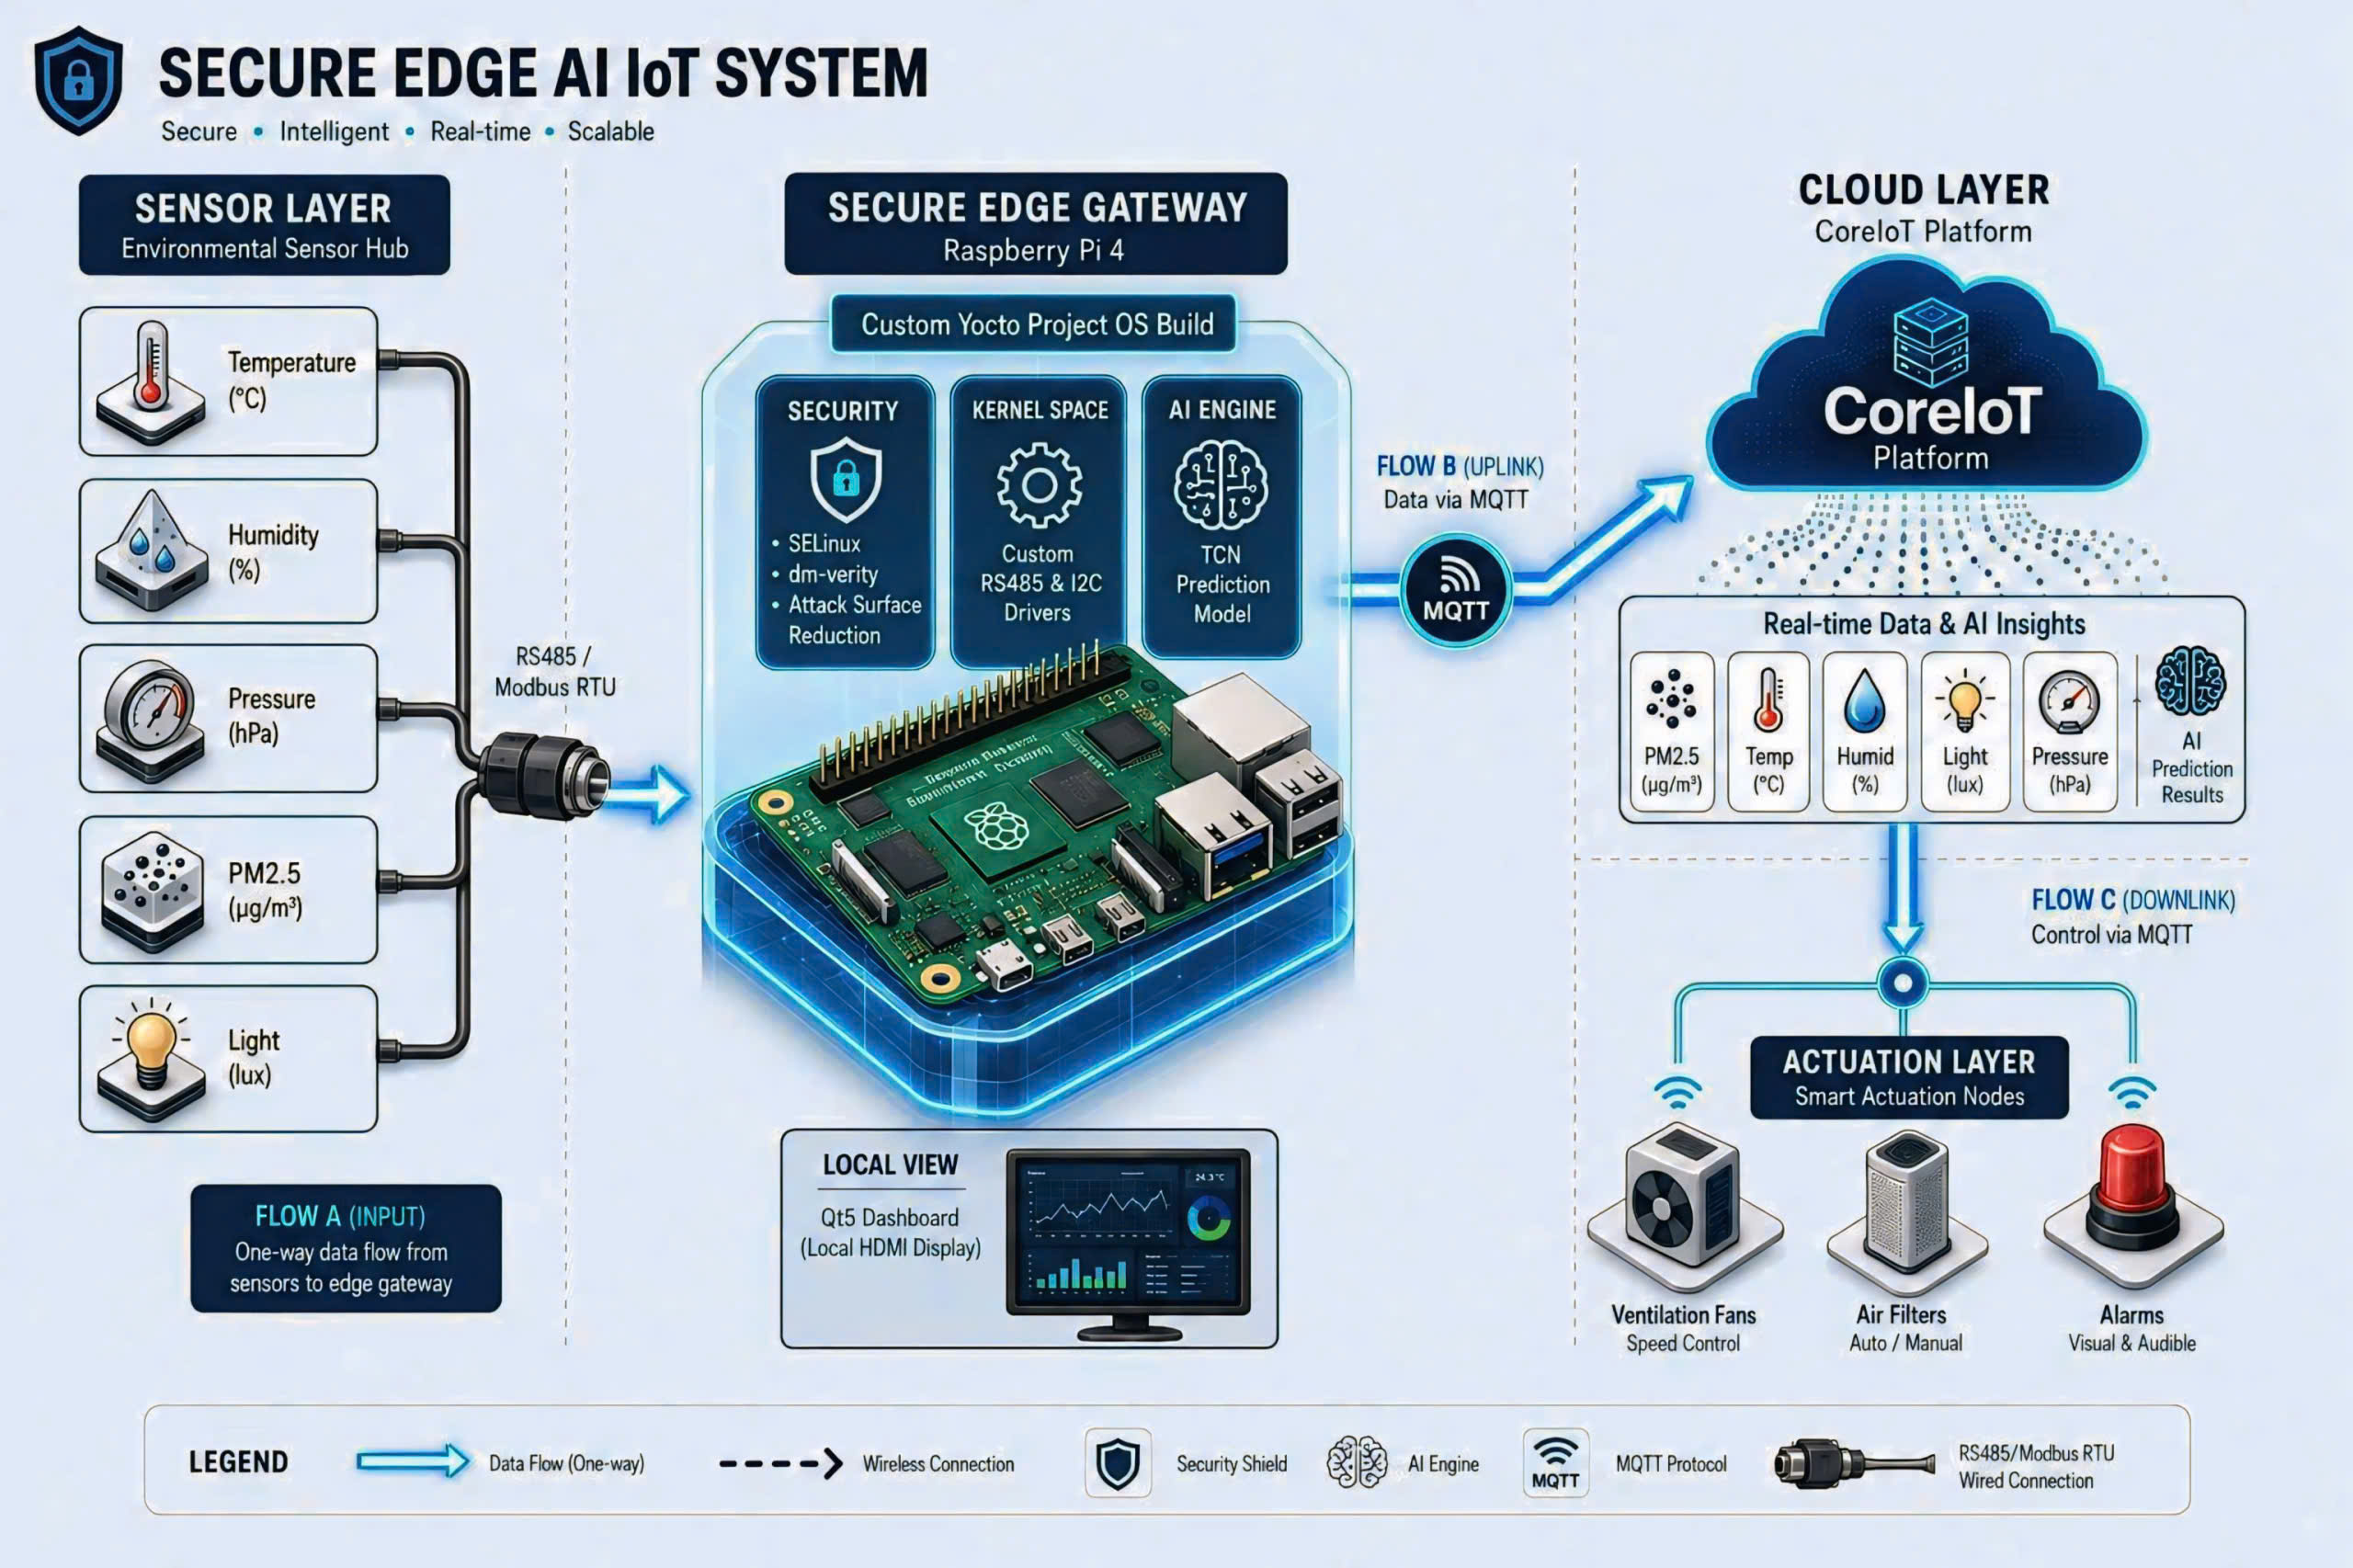
\includegraphics[width=0.9\linewidth]{image/kientructongquan.jpg}
    \caption{Kiến trúc tổng thể của hệ thống}
    \label{fig:placeholder}
\end{figure}

\section{Phạm vi và giới hạn nghiên cứu}

Đề tài tập trung xây dựng nền tảng Linux nhúng (Embedded Linux) dành cho các ứng dụng công nghiệp và IoT (Internet of Things) dựa trên Yocto Project. Hệ điều hành được phát triển theo hướng tùy biến cao, phù hợp với thiết bị biên (Edge Device) có tài nguyên phần cứng giới hạn. Trên cơ sở đó, nội dung nghiên cứu bao gồm cơ chế build image, quản lý gói phần mềm (package) và tích hợp Linux Device Driver trong môi trường Yocto nhằm đáp ứng yêu cầu giao tiếp, điều khiển phần cứng trên hệ thống nhúng.

Bên cạnh việc phát triển nền tảng, đề tài còn đi sâu vào các thành phần cốt lõi của Linux Kernel như Kernel Module, Device Tree và cơ chế quản lý module lúc runtime. Những kiến thức này là nền tảng cho việc phát triển và tích hợp driver trong hệ thống Linux nhúng, đồng thời nâng cao khả năng làm chủ hệ thống ở mức thấp đối với các bài toán công nghiệp.

Về mặt bảo mật, đề tài tích hợp một số cơ chế phổ biến trong Linux Embedded như Secure Boot, dm-verity và fscrypt nhằm tăng cường bảo vệ firmware, filesystem và dữ liệu trên thiết bị. Hệ thống cũng hỗ trợ các chức năng quản lý dịch vụ và cấu hình cơ bản để đảm bảo vận hành ổn định trong thực tế.

Về truyền thông và IoT, nền tảng triển khai cơ chế kết nối giữa thiết bị và hệ thống quản lý qua các giao thức MQTT và HTTP. Hệ thống có khả năng thu thập, xử lý và truyền dữ liệu cảm biến theo thời gian thực, đồng thời xây dựng cơ chế giám sát và cảnh báo phục vụ quản lý thiết bị trong môi trường công nghiệp.

Để kiểm chứng khả năng ứng dụng thực tế, đề tài triển khai mô hình quản lý kho thông minh dựa trên nền tảng đã xây dựng. Mô hình này tập trung giám sát các thông số môi trường như nhiệt độ, độ ẩm và trạng thái hoạt động của kho hàng, kèm theo dashboard giám sát và backend cơ bản để lưu trữ, hiển thị và quản lý dữ liệu thiết bị.

Tuy nhiên, do giới hạn về thời gian, tài nguyên và phạm vi nghiên cứu, đề tài mới chỉ dừng lại ở mô hình thử nghiệm, chưa được đánh giá trên quy mô công nghiệp lớn. Các bài toán chuyên sâu như tối ưu logistics, quản lý chuỗi cung ứng hay tích hợp hệ thống ERP/WMS hoàn chỉnh chưa được đề cập. Ngoài ra, đề tài chưa nghiên cứu các cơ chế bảo mật phần cứng nâng cao (TPM, HSM) hoặc giải pháp chống tấn công vật lý. Các kỹ thuật trí tuệ nhân tạo và machine learning phục vụ dự đoán, tối ưu vận hành hệ thống cũng chưa được tích hợp trong phạm vi hiện tại.

\section{Bố cục luận văn}

Luận văn được tổ chức thành 6 chương với nội dung chính như sau:

\begin{itemize}

    \item \textbf{Chương 1: Phần mở đầu} \\ 
    Trình bày bối cảnh nghiên cứu, lý do chọn đề tài, mục tiêu nghiên cứu, phạm vi triển khai và bố cục tổng thể của luận văn.

    \item \textbf{Chương 2: Tổng quan dự án} \\ 
    Trình bày tổng quan về Linux Embedded, Yocto Project, Industrial IoT và các công nghệ liên quan đến hệ thống nhúng và tự động hóa công nghiệp.

    \item \textbf{Chương 3: Cơ sở lý thuyết} \\ 
    Trình bày các cơ sở lý thuyết phục vụ cho việc xây dựng hệ thống, bao gồm Yocto Project, BitBake, Linux Kernel, Linux Device Driver, Kernel Module và các cơ chế tích hợp driver trong Linux Embedded.

    \item \textbf{Chương 4: Thiết kế hệ thống} \\ 
    Phân tích yêu cầu hệ thống, xây dựng kiến trúc tổng thể và thiết kế các thành phần kỹ thuật như Linux Embedded Platform, Driver phần cứng, bảo mật hệ thống và cơ chế giao tiếp IoT.

    \item \textbf{Chương 5: Triển khai và đánh giá} \\ 
    Trình bày quá trình triển khai hệ điều hành bằng Yocto Project, xây dựng Linux Device Driver, tích hợp MQTT/HTTP, triển khai hệ thống giám sát và đánh giá kết quả hoạt động của hệ thống.

    \item \textbf{Chương 6: Kết luận và hướng phát triển} \\ 
    Tổng kết các kết quả đạt được, đánh giá ưu điểm và hạn chế của hệ thống, đồng thời đề xuất các hướng phát triển trong tương lai.

\end{itemize}